\documentclass[12pt]{article}

\usepackage[utf8]{inputenc}
\usepackage{datetime}
\usepackage{amsthm}
\usepackage{amsmath}
\usepackage{amssymb}
\usepackage{enumitem}
\usepackage[english]{babel}
\usepackage{matlab-prettifier}
\usepackage{graphicx}
\usepackage[makeroom]{cancel}
\usepackage{afterpage}
\usepackage{capt-of}
\usepackage{bm}
\usepackage{float}

\DeclareMathOperator*{\argmin}{arg\,min}
\DeclareMathOperator*{\argmax}{arg\,max}

\newcommand\independent{\protect\mathpalette{\protect\independenT}{\perp}}
\def\independenT#1#2{\mathrel{\rlap{$#1#2$}\mkern2mu{#1#2}}}

\newtheoremstyle{colon}{\topsep}{\topsep}{}{}{\bfseries}{:}{ }{}
\theoremstyle{colon}
\newtheorem{exercise}{Exercise}
\newtheorem*{answer}{Answer}

\title{ELE 535: Machine Learning and Pattern Recognition \\ Homework 1}
\author{Zachary Hervieux-Moore}

\newdate{date}{24}{09}{2018}
\date{\displaydate{date}}

\begin{document}

\maketitle

\clearpage

\begin{exercise}
  Consider the training data $\{(x_j, y_j)\}_{j=1}^m$, with $x_j \in \mathbb{R}^n$ and $y_j \in \{0,1\}$. Assume the training data has an equal number of examples from each class. Hence the estimated prior probabilities of each class are equal. The nearest centroid classifer has

  \begin{gather*}
    \hat{y}(x) = \begin{cases} 
      1, & \text{if } \lVert x - \hat{\mu}_1 \rVert_2 < \lVert x - \hat{\mu}_0 \rVert_2; \\
      0, & \text{o.w.}
    \end{cases}
  \end{gather*}

  \begin{enumerate}[label=\alph*)]
    \item Show that the nearest centroid classifier is a linear classifier with
      \begin{gather*}
        w = (\hat{\mu}_0 - \hat{\mu}_1) \\
        b = (\hat{\mu}_1 - \hat{\mu}_0)^T \frac{(\hat{\mu}_1 + \hat{\mu}_0)}{2}
      \end{gather*}

    \item Show that the classifier can also be written as
      \begin{gather*}
        \hat{y}(x) = \begin{cases} 
          1, & \text{if } \langle \hat{\mu}_0 - \hat{\mu}_1, x - \hat{\mu} \rangle < 0; \\
          0, & \text{o.w.}
        \end{cases}
      \end{gather*}

      Here $\hat{\mu} \triangleq \frac{1}{m} \sum_{i=1}^m x_i$ denotes the mean of the training examples. So the result of classification depends solely on the sign of a inner product.

    \item By neatly sketching the vectors $x - \hat{\mu}$ and $\hat{\mu}_0 - \hat{\mu}_1$, give a geometric interpretation of this classifier.

    \item Suppose we first center the training data by subtracting $\hat{\mu}$ from each training example. Determine the form of the nearest centroid classifier for the centered training data.
  \end{enumerate}
\end{exercise}

\begin{answer}
  \

  \begin{enumerate}[label=\alph*)]
    \item We define a linear classifier as:
      \begin{align*}
        &w^T x + b < 0 \\
        &\Longleftrightarrow (\hat{\mu}_0 - \hat{\mu}_1)^T x + (\hat{\mu}_1 - \hat{\mu}_0)^T \frac{(\hat{\mu}_1 + \hat{\mu}_0)}{2} < 0 \\
        &\Longleftrightarrow x^T x - 2 \hat{\mu}_1^T x + \hat{\mu}_1^T \hat{\mu}_1 < x^T x - 2 \hat{\mu}_0^T x + \hat{\mu}_0^T \hat{\mu}_0 \\
        &\Longleftrightarrow \lVert x - \hat{\mu}_1 \rVert_2^2 < \lVert x - \hat{\mu}_0 \rVert_2^2 \\
        &\Longleftrightarrow \lVert x - \hat{\mu}_1 \rVert_2 < \lVert x - \hat{\mu}_0 \rVert_2
      \end{align*}
      where I added $x^T x$ to both sides in the second step.

    \item By assumption of equal class sizes, we have that
      \begin{gather*}
        \hat{\mu} = \frac{\hat{\mu}_1 + \hat{\mu}_0}{2}
      \end{gather*}
      Then, our linear classifier from above becomes
      \begin{align*}
        & (\hat{\mu}_0 - \hat{\mu}_1)^T x + (\hat{\mu}_1 - \hat{\mu}_0)^T \frac{(\hat{\mu}_1 + \hat{\mu}_0)}{2} < 0 \\
        &\Longleftrightarrow (\hat{\mu}_0 - \hat{\mu}_1)^T x + (\hat{\mu}_1 - \hat{\mu}_0)^T \hat{\mu} < 0 \\
        &\Longleftrightarrow \langle \hat{\mu}_0 - \hat{\mu}_1, x - \hat{\mu} \rangle < 0
      \end{align*}
      Which, by equivalence of part a), is equivalent to the nearest centroid classifier.

    \item Sketch shown below in Figure 1. Essentially, the geometric interpretation is that if the angle between $x - \hat{\mu}$ and $\hat{\mu}_0 - \hat{\mu}_1$ is obtuse (or the dot product is negative), then the point $x$ lies on the side of the mean closer to $\hat{\mu}_1$ and hence closer to $\hat{\mu}_1$. In my example, the angle is acute and therefore $x$ is closer to $\hat{\mu}_0$ and should be classified as such.
      \begin{figure}[H]
        \centering
          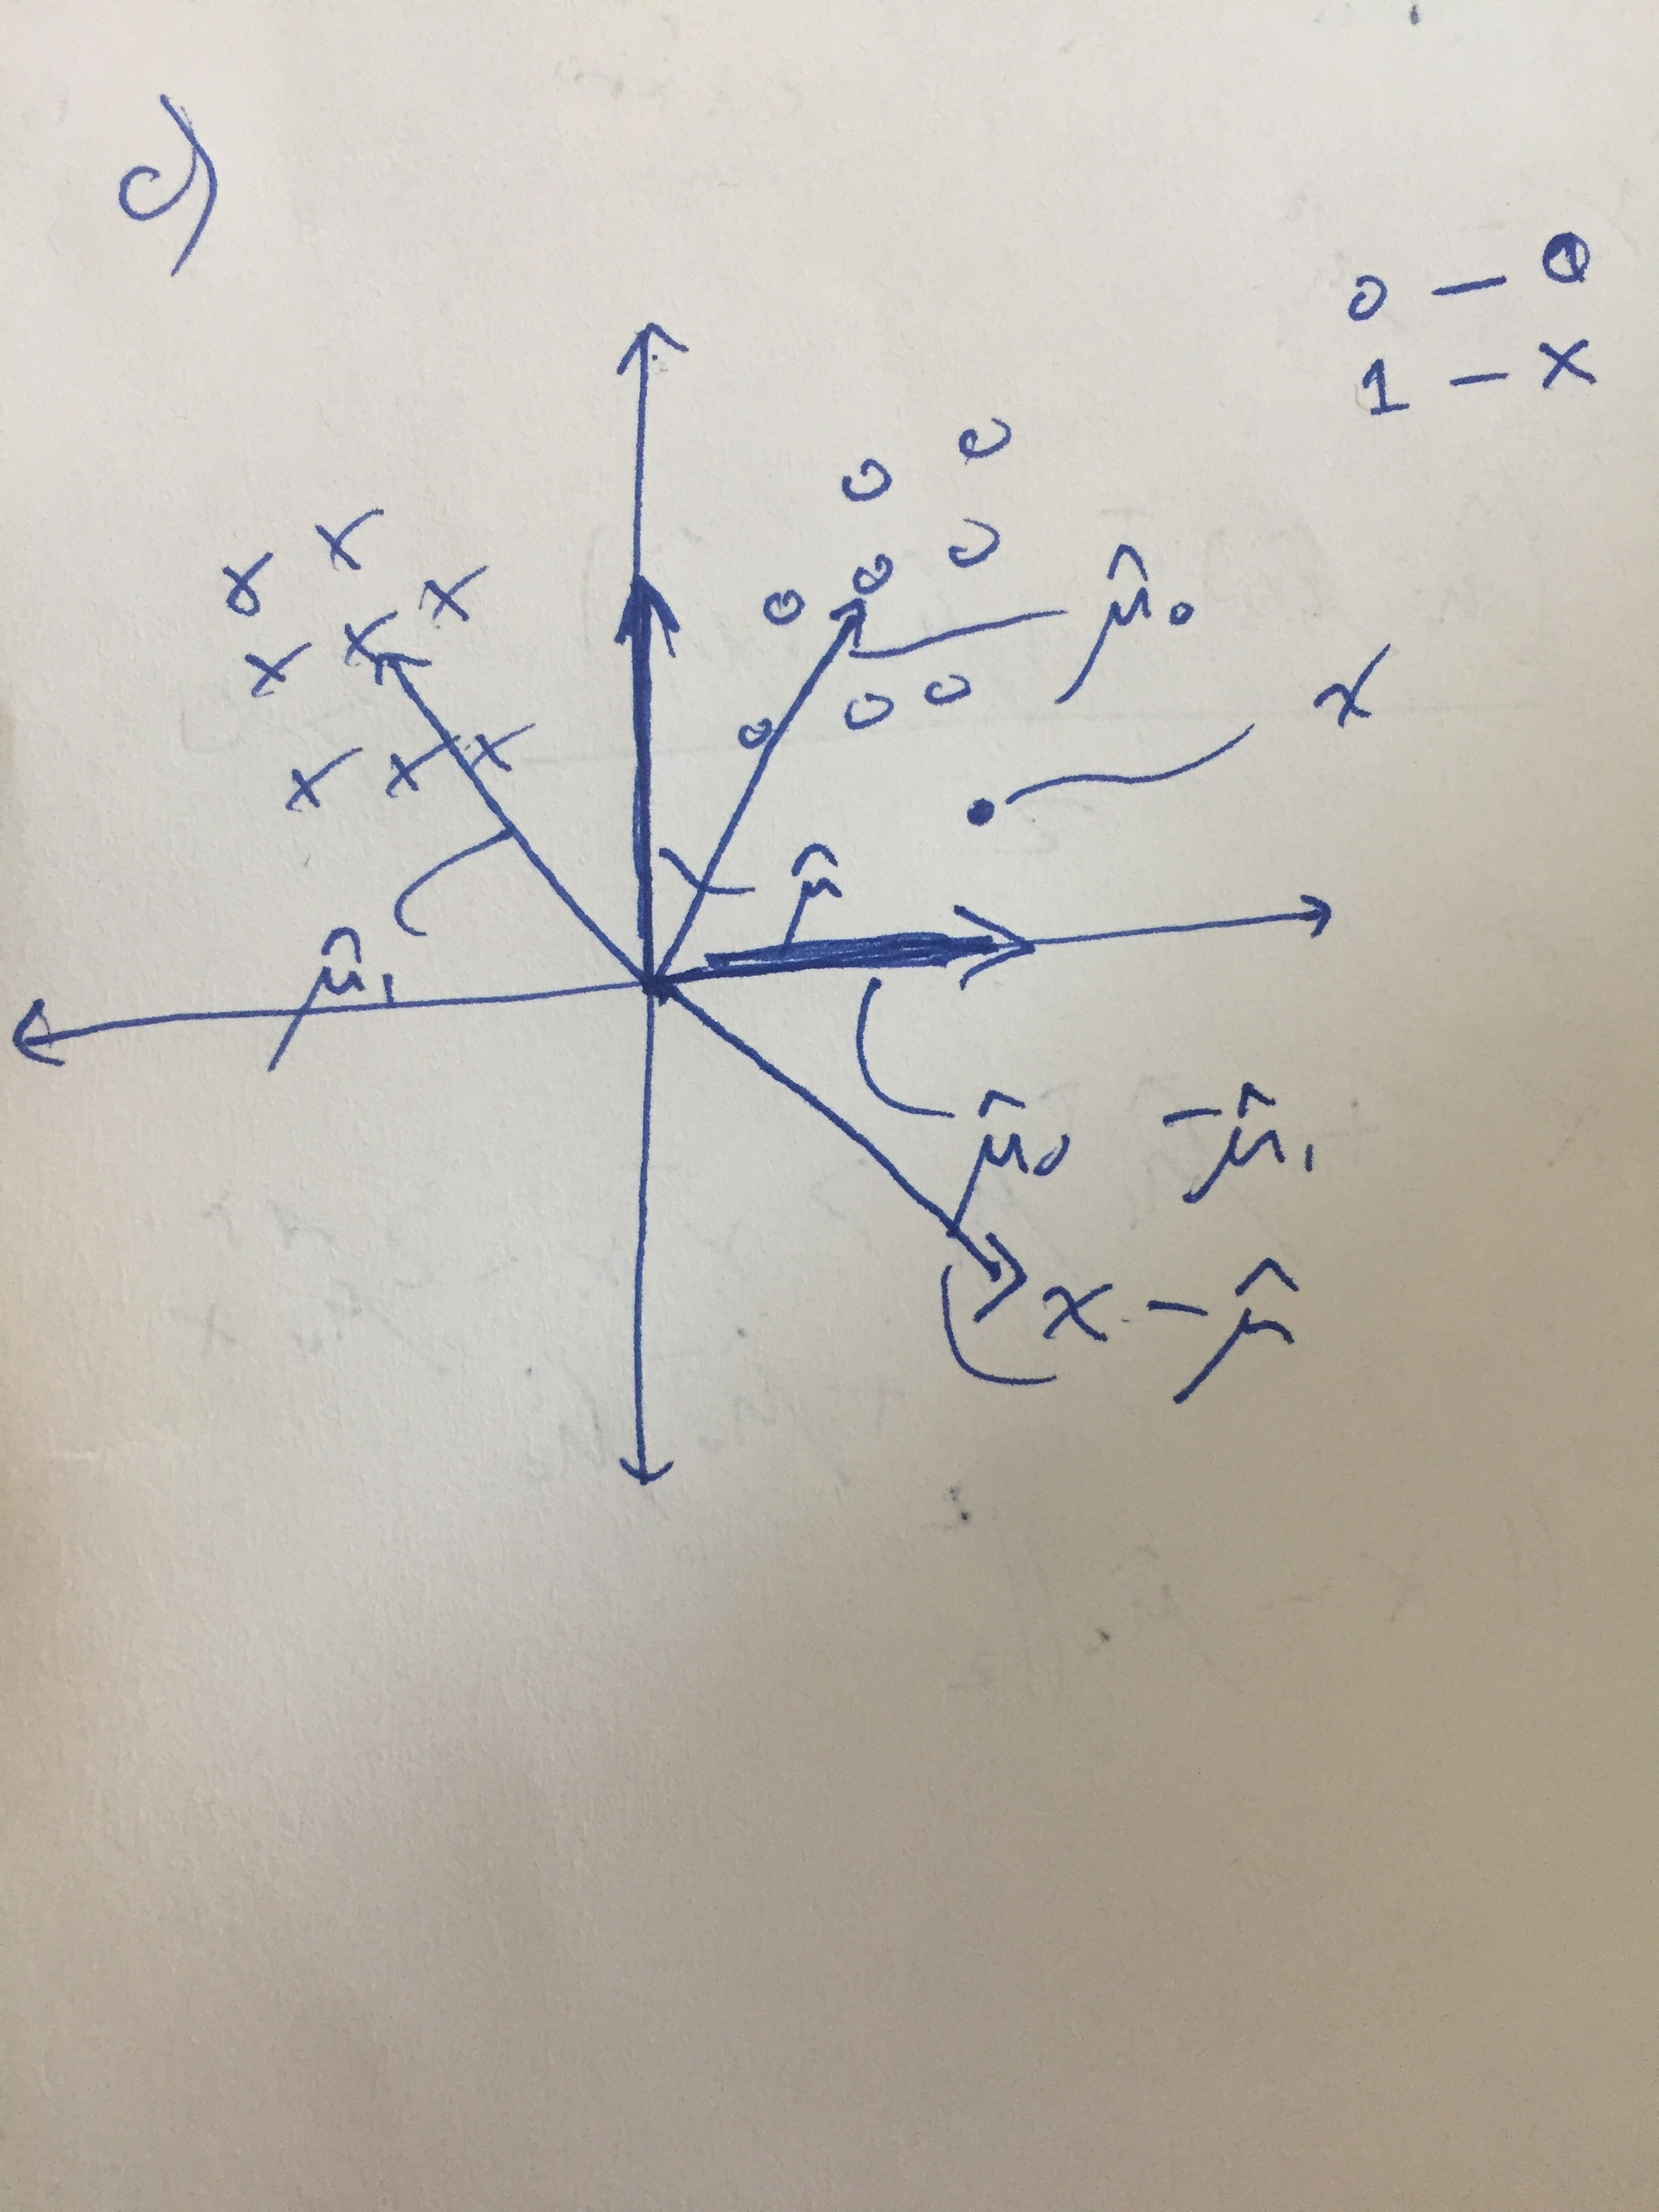
\includegraphics[width=\textwidth]{q1c}
        \caption{Sktech of $x - \hat{\mu}$ and $\hat{\mu}_0 - \hat{\mu}_1$}
      \end{figure}

    \item We define
      \begin{gather*}
        \tilde{x} = x - \hat{\mu}
      \end{gather*}
      Then, using our characterization from part b), we get
      \begin{align*}
        & \langle \hat{\mu}_0 - \hat{\mu}_1, x - \hat{\mu} \rangle \\
        &= \langle (\hat{\mu}_0 - \hat{\mu}) - (\hat{\mu}_1 - \hat{\mu}), x - \hat{\mu} \rangle \\
        &= \langle \tilde{\mu}_0 - \tilde{\mu}_1, \tilde{x} \rangle
      \end{align*}
      So our nearest centroid classifier becomes

      \begin{gather*}
        \hat{y}(x) = \begin{cases} 
          1, & \langle \tilde{\mu}_0 - \tilde{\mu}_1, \tilde{x} \rangle; \\
          0, & \text{o.w.}
        \end{cases}
      \end{gather*}

  \end{enumerate}
\end{answer}

\clearpage

\begin{exercise}
  For a $n \times m$ real matrix $X$ show that:

  \begin{enumerate}[label=\alph*)]
    \item $\mathcal{R}(X) \triangleq \{ z \mathbb{R}^n: z = Xw, \text{ for } w \in \mathbb{R}^m \}$ is a subspace of $\mathbb{R}^n$.

    \item $\mathcal{N}(X) \triangleq \{ a \in \mathbb{R}^m: Xa = \bm{0} \}$ is a subspace of $\mathbb{R}^m$.
  \end{enumerate}
\end{exercise}

\begin{answer}
  \

  \textbf{Note: } To show $S$ is a subspace, one must show 3 things:
  \begin{enumerate}[label=\roman*)]
    \item $\bm{0} \in S$
    \item if $x, y \in S$ then $x + y \in S$
    \item if $x \in S$ and $\alpha \in \mathbb{R}$ then $\alpha x \in S$
  \end{enumerate}

  \begin{enumerate}[label=\alph*)]
    \item 
      \begin{enumerate}[label=\roman*)]
        \item By picking $w = \bm{0}_m$ we have that $z = X w = X \bm{0} = \bm{0}_n$ and so $\bm{0}_n \in \mathcal{R}(X)$

        \item Pick $z_1, z_2 \in \mathcal{R}(X)$ then we have
          \begin{gather*}
            z_1 + z_2 = X w_1 + X w_2 = X (w_1 + w_2)
          \end{gather*}
          and since $(w_1 + w_2) \in \mathbb{R}^m$ we have $z_1 + z_2 \in \mathcal{R}(X)$

        \item Pick $z\in \mathcal{R}(X)$ and $\alpha \in \mathbb{R}$ then we have
          \begin{gather*}
            \alpha z = \alpha X w = X (\alpha w)
          \end{gather*}
          and since $(\alpha w) \in \mathbb{R}^m$ we have $\alpha z \in \mathcal{R}(X)$
      \end{enumerate}

    \item 
      \begin{enumerate}[label=\roman*)]
        \item By picking $a = \bm{0}_m$ we have that $X a = X \bm{0}_m = \bm{0}_n$ and so $\bm{0}_m \in \mathcal{N}(X)$

        \item Pick $a_1, a_2 \in \mathcal{N}(X)$ then we have
          \begin{gather*}
            X(a_1 + a_2) = X a_1 + X a_2 = \bm{0}_n + \bm{0}_n = \bm{0}_n
          \end{gather*}
          and so we have $a_1 + a_2 \in \mathcal{N}(X)$

        \item Pick $a\in \mathcal{N}(X)$ and $\alpha \in \mathbb{R}$ then we have
          \begin{gather*}
            X (\alpha a) = \alpha X a = \alpha \bm{0}_n = \bm{0}_n
          \end{gather*}
          and so we have $\alpha a \in \mathcal{N}(X)$
      \end{enumerate}
  \end{enumerate}
\end{answer}

\clearpage

\begin{exercise}
  \ 

  \begin{enumerate}[label=\alph*)]
    \item Let $A_j \in \mathbb{R}^{n_j \times m}$ and $\mathcal{N}_j = \{ x \in \mathbb{R}^m: A_j x = \bm{0} \}$, $j = 1, 2$. Show that $\mathcal{N}_1 \cap \mathcal{N}_2$ is a subspace of $\mathbb{R}^m$. Give a similar matrix equation for this subspace.

    \item Let $A_j \in \mathbb{R}^{n \times m_j}$ and $\mathcal{R}_j = \{ y \mathbb{R}^n: y = A_j x, \text{ with } x \in \mathbb{R}^{m_j} \}$, $j = 1, 2$. Show that $\mathcal{R}_1 + \mathcal{R}_2 = \{y_1 + y_2: y \in \mathcal{R}_1, y_2 \in \mathcal{R}_2 \}$ is a subspace of $\mathbb{R}^n$. Give a similar matrix equation for this subspace.
  \end{enumerate}
\end{exercise}

\begin{answer}
  \
  
  \textbf{Note: } To show $S$ is a subspace, one must show 3 things:
  \begin{enumerate}[label=\roman*)]
    \item $\bm{0} \in S$
    \item if $x, y \in S$ then $x + y \in S$
    \item if $x \in S$ and $\alpha \in \mathbb{R}$ then $\alpha x \in S$
  \end{enumerate}

  \begin{enumerate}[label=\alph*)]
    \item 
      \begin{enumerate}[label=\roman*)]

        \item By question Q2  part b), we know that $\bm{0}_m \in \mathcal{N}_j$ for $j = 1, 2$ and so $\bm{0}_m \in \mathcal{N}_1 \cap \mathcal{N}_2$.

        \item Pick $x_1, x_2 \in \mathcal{N}_1 \cap \mathcal{N}_2$ then we have
          \begin{gather*}
            A_j (x_1 + x_2) = A_j x_1 + A_j x_2 = \bm{0}_n
          \end{gather*}
          For both $j = 1, 2 $ and since $(x_1 + x_2) \in \mathbb{R}^m$ we have $x_1 + x_2 \in \mathcal{N}_1 \cap \mathcal{N}_2$

        \item Pick $x \in \mathcal{N}_1 \cap \mathcal{N}_2$ and $\alpha \in \mathbb{R}$ then we have
          \begin{gather*}
            A_j (\alpha x) = \alpha A_j x = \alpha \bm{0}_n = \bm{0}_n
          \end{gather*}
          For both $j = 1, 2 $ and since $(\alpha x) \in \mathbb{R}^m$ we have $\alpha x \in \mathcal{N}_1 \cap \mathcal{N}_2$
      \end{enumerate}

      The similar matrix equation is 
      
      \begin{gather*}
        \mathcal{N}_1 \cap \mathcal{N}_2 = \left\{ x \in \mathbb{R}^m: \begin{bmatrix} A_1 & \bm{0}_{n_1 \times m} \\ \bm{0}_{n_2 \times m} & A_2\end{bmatrix} \begin{bmatrix} x \\ x \end{bmatrix} = \bm{0}_{n_1 + n_2} \right\}
      \end{gather*}

    \item 
      \begin{enumerate}[label=\roman*)]

        \item By question Q2  part a), we know that $\bm{0}_n \in \mathcal{R}_j$ for $j = 1, 2$ and so $\bm{0}_n \in \mathcal{R}_1 + \mathcal{R}_2$ as $\bm{0}_n + \bm{0}_n = \bm{0}_n$.

        \item Pick $a, b \in \mathcal{R}_1 + \mathcal{R}_2$ then we also have for some $a_1, b_1 \in \mathcal{R}_1$ and $a_2, b_2 \in \mathcal{R}_2$ where
          \begin{gather*}
            a = a_1 + a_2 = A_1 x_1 + A_2 x_2 \\
            b = b_1 + b_2 = A_1 x_1' + A_2 x_2' \\
            a + b = a_1 + b_1 + a_2 + b_2 = A_1 (x_1 + x_1') + A_2 (x_2 + x_2')
          \end{gather*}
          As all the dimensions are appropriate and everything is in the proper spaces, we have $a + b \in \mathcal{R}_1 + \mathcal{R}_2$.

        \item Pick $a \in \mathcal{R}_1 + \mathcal{R}_2$ and $\alpha \in \mathbb{R}$ then for some $a_1 \in \mathcal{R}_1$ and $a_2 \in \mathcal{R}_2$
          \begin{gather*}
            a = a_1 + a_2 = A_1 x_1 + A_2 x_2 \\
            \alpha a = \alpha A_1 x_1 + \alpha A_2 x_2 = A_1 (\alpha x_1) + A_2 (\alpha x_2)
          \end{gather*}
          As all the dimensions are appropriate and everything is in the proper spaces, we have $\alpha a \in \mathcal{R}_1 + \mathcal{R}_2$.
      \end{enumerate}

      The similar matrix equation is 
      
      \begin{gather*}
        \mathcal{R}_1 + \mathcal{R}_2 = \left\{ y \in \mathbb{R}^n: y = \begin{bmatrix} A_1 & A_2 \end{bmatrix} \begin{bmatrix} w_1 \\ w_2 \end{bmatrix} \text{ for } \begin{bmatrix} w_1 \\ w_2 \end{bmatrix} \in \mathbb{R}^{m_1 + m_2} \right\}
      \end{gather*}
  \end{enumerate}
\end{answer}

\clearpage

\begin{exercise}
  For $A, B \in \mathbb{R}^{m \times n}$, the inner product of $A$ and $B$ is $\langle A, B \rangle \triangleq \sum_i \sum_j A_{i,j} B_{i,j}$. Show that $\langle A, B \rangle = \text{trace} (A^T B)$.
\end{exercise}

\begin{answer}
  We do this by direct computation.
  \begin{gather*}
    \text{trace}(A^T B) = \sum_j (A^T B)_{j, j} = \sum_j \sum_i A_{j,i}^T B_{i,j} \\
    = \sum_j \sum_i A_{i,j} B_{i,j} = \sum_i \sum_j A_{i,j} B_{i,j} = \langle A, B \rangle
  \end{gather*}
  Where the sum can be exchanged because they are both finite.
\end{answer}

\clearpage

\begin{exercise}
  Consider the vector space of real $n \times n$ matrices. Let $\mathcal{S}$ and $\mathcal{A}$ denote the subsets of symmetric ($P^T = P$) and antisymmetric ($A^T = -A$) matrices, respectively. Show that $\mathcal{S}$ and $\mathcal{A}$ are subspaces of $\mathbb{R}^{n \times n}$ and that $\mathcal{S}^{\perp} = \mathcal{A}$. Hence $\mathbb{R}^{n \times n} = \mathcal{S} \oplus \mathcal{A}$
\end{exercise}

\begin{answer}
  \
  
  \textbf{Note: } To show $S$ is a subspace, one must show 3 things:
  \begin{enumerate}[label=\roman*)]
    \item $\bm{0} \in S$
    \item if $x, y \in S$ then $x + y \in S$
    \item if $x \in S$ and $\alpha \in \mathbb{R}$ then $\alpha x \in S$
  \end{enumerate}

  We start with symmetric matrices.

  \begin{enumerate}[label=\roman*)]
    \item The all 0 matrix is clearly symmetric.
    \item Pick $P_1, P_2 \in \mathcal{S}$ then we have that
      \begin{gather*}
        (P_1 + P_2)_{i,j} = (P_1 + P_2)_{j,i}
      \end{gather*}
      since $P_{1_{i,j}} = P_{1_{i,j}}$ and $P_{2_{i,j}} = P_{2_{i,j}}$ and so $P_1 + P_2 \in \mathcal{S}$.
    \item Pick $P \in \mathcal{S}$ and $\alpha \in \mathbb{R}$ then we have that
      \begin{gather*}
        (\alpha P)^T = \alpha P^T = \alpha P
      \end{gather*}
      and so $\alpha P \in \mathcal{S}$
  \end{enumerate}

  So symmetric matrices form a subspace. Very similarly for antisymmetric matrices.

  \begin{enumerate}[label=\roman*)]
    \item The all 0 matrix is clearly antisymmetric.
    \item Pick $A_1, A_2 \in \mathcal{A}$ then we have that
      \begin{gather*}
        (A_1 + A_2)_{i,j} = -(A_1 + A_2)_{j,i}
      \end{gather*}
      since $A_{1_{i,j}} = -A_{1_{i,j}}$ and $A_{2_{i,j}} = -A_{2_{i,j}}$ and so $A_1 + A_2 \in \mathcal{S}$.
    \item Pick $A \in \mathcal{A}$ and $\alpha \in \mathbb{R}$ then we have that
      \begin{gather*}
        (\alpha A)^T = \alpha A^T = -\alpha A
      \end{gather*}
      and so $\alpha A \in \mathcal{A}$.
  \end{enumerate}

  So antisymmetric matrices form a subspace. Now to show that they are orthogonal complements of each other. We first define the complement of $\mathcal{S}$.
  \begin{gather*}
    \mathcal{S}^\perp \triangleq \{ X: \forall \ P \in \mathcal{S}, \langle X, P \rangle = \bm{0} \}
  \end{gather*}

  From this, it is trivial to see that $\mathcal{A} \subseteq \mathcal{S}^\perp$ because the inner product of a symmetric and antisymmetric matrix will yield $\bm{0}$ by the definition of the sum shown in question 4. Similarly, showing $\mathcal{S}^\perp \subseteq \mathcal{A}$ is easy to see from the summation. For $\langle X, P \rangle = \bm{0}$, we need
  \begin{gather*}
    \sum_i \sum_j X_{i,j} P_{i,j} = \bm{0}
  \end{gather*}
  By picking the all 0's symmetric matrix, we get that the diagonal of $X = 0$. Furthermore, by picking symmetric matrices with 0's every where except for one entry (and its pair) to be 1, we get that $X_{i,j} + X_{j,i} = 0$ or $X_{i,j} = -X_{j,i}$. Thus, we have that $X \in \mathcal{A}$. Thus we have shown both sides are subsets of each other and conclude that $\mathcal{A} = \mathcal{S}^\perp$ and that this means $\mathbb{R}^{n \times n} = \mathcal{S} \oplus \mathcal{A}$.
\end{answer}

\end{document}